\documentclass[10pt,a4paper]{article}
\usepackage[utf8]{inputenc}
\usepackage{amsmath}
\usepackage{amsfonts}
\usepackage{amssymb}
\usepackage{algorithmic}
\usepackage{amsthm}
\usepackage{physics}
\usepackage{mathtools}
\DeclarePairedDelimiter{\ceil}{\lceil}{\rceil}



\newtheorem{theorem}{\bf Theorem}
\newtheorem{todo}{\bf Todo}
\newtheorem{remark}{\bf Remark}
\newtheorem{corollary}{\bf Corollary}
\newtheorem{definition}{\bf Definition}
\newtheorem{lemma}{\bf Lemma}
\newtheorem{proposition}[theorem]{\bf Proposition}

\newenvironment{sproof}{%
  \renewcommand{\proofname}{Sketch of Proof}\proof}{\endproof}

\begin{document}

\section{Fixed and Relative Bouncing Results}

\begin{figure}[thpb]
  \centering
  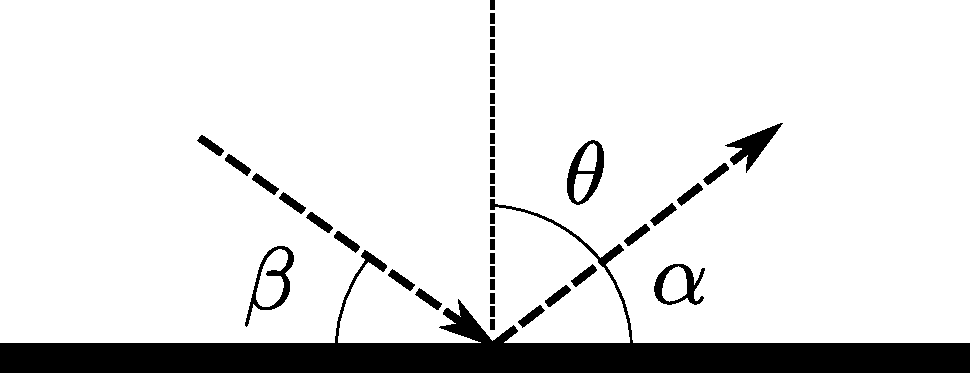
\includegraphics[width=0.4\textwidth]{beTheAlp.pdf}
  \caption{Angle of incidence $\beta$, angle of departure $\alpha$ and bouncing angle $\theta$.}
  \label{fig:fixed_boun}
\end{figure}

\begin{definition}
\textbf{\emph{Fixed bouncing}} consists in the robot driving in a straight line until encountering $\delta P$, then make the robot rotate until its heading is at an angle $\theta$ clockwise of the inward-facing boundary normal.
 \end{definition}

\begin{figure}[thpb]
  \centering
  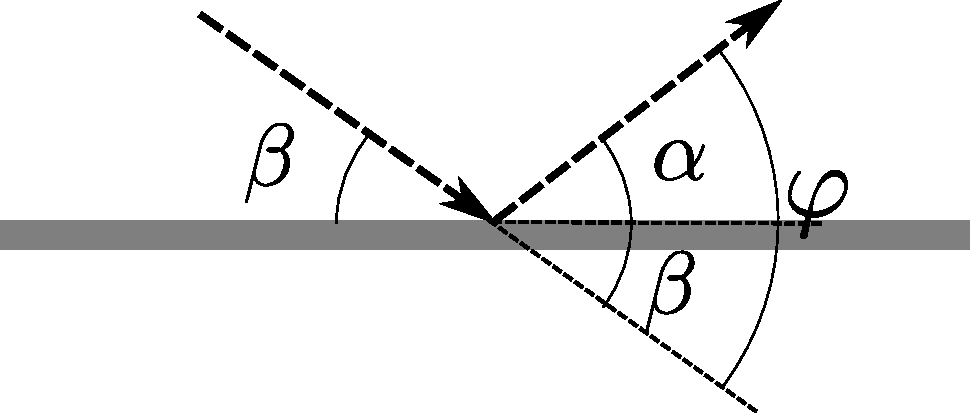
\includegraphics[width=0.4\textwidth]{beThePhi.pdf}
  \caption{Angle of incidence $\beta$, angle of departure $\alpha$ and bouncing angle $\varphi$.}
  \label{fig:relative_boun}
\end{figure}

\begin{definition}
\textbf{\emph{Relative bouncing}} consists in the robot driving in a straight line until encountering $\delta P$, then make the robot rotate an angle $\varphi$ from its current orientation.
 \end{definition} 

\begin{figure}[thpb]
  \centering
  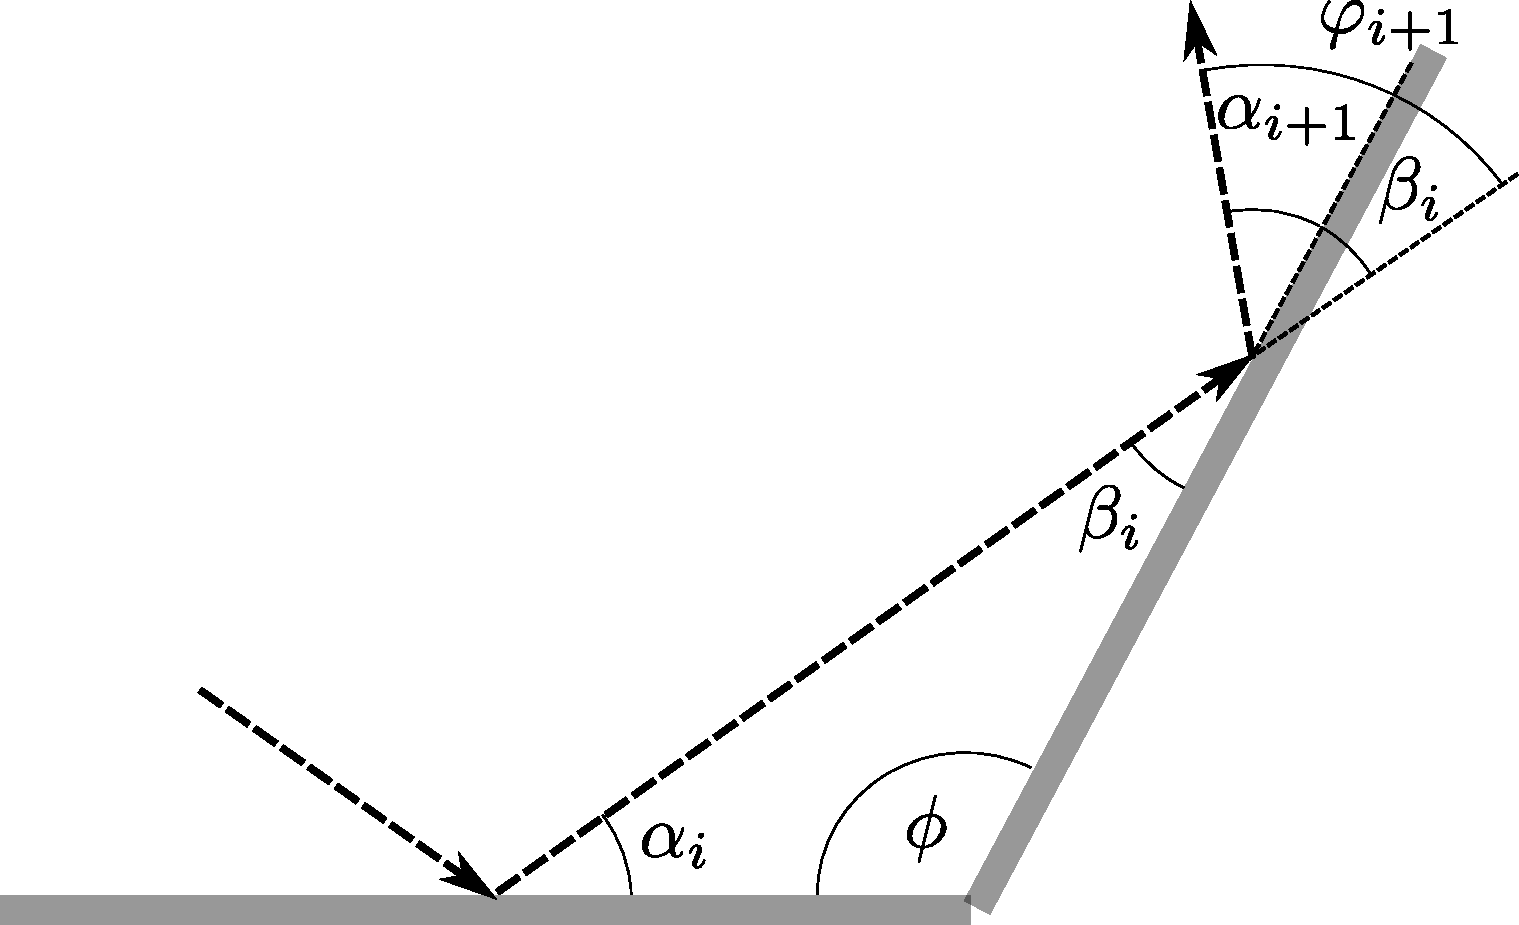
\includegraphics[width=0.5\textwidth]{fixedRelativeEqui.pdf}
  \caption{Equivalence between fixed bouncing and relative bouncing.}
  \label{fig:equiv}
\end{figure}

\begin{proposition} \label{Proposition:equivalency}
In every regular $n$-sided polygon with interior angle $\phi = (n - 2)\pi/n$, there exist an angle $\varphi$ that makes relative bouncing equivalent to fixed bouncing. Moreover, $\varphi = \pi - \phi$. 
\end{proposition}
\begin{proof}
We proceed by induction. Consider the angle of departure $\alpha_i$ after the robot bounces from $\delta P$ for the $i$-\textit{th} time. In the fixed bouncing scheme, the robot always bounces from $\delta P$ at a fixed angle $\theta$, which implies $\alpha_i$ to remain equal in each bounce, that is, $\alpha_{i+1} = \alpha_{i}$. Referring to Figure~\ref{fig:equiv}, a departing angle $\alpha_i$ yields a angle of incidence $\beta_{i}$. If we require $\alpha_{i+1} = \alpha_{i}$, then an equivalent relative bouncing law should subsequently apply a bounce angle $\varphi_{i+1}=\alpha_{i+1}+\beta{i}=\alpha_{i}+\beta{i}$. From the triangle whose interior angles are $\alpha_{i}$, $\beta{i}$ and $\phi$, we get that $\alpha_{i} + \beta{i} = \pi - \phi$, hence, $\varphi_{i+1} = \pi - \phi$, which is independent of index $i$. As the base case, consider that the robot encounters  $\delta P$ for the first time with an angle $\beta_{0}$; if the robot starts a relative bouncing scheme with an angle $\varphi_{1} = \pi - \phi$ and keeps bouncing with $\varphi_{i}= \pi - \phi$ (assuming that this bouncing keeps the robot inside $P$), then it will produce a fixed bouncing behaviour with a fixed $\theta=\phi + \beta_0 - \pi/2$. The result follows. 
\end{proof}

\begin{corollary} \label{Lemma:equivalency}
The angle $\varphi = \pi - \phi$ that makes relative bouncing equivalent to fixed bouncing is unique for a regular $n$-sided polygon, and for a given angle of incidence $\beta_0$ it yields at most one bouncing angle $\theta$. 
\end{corollary}


\section{Fixed Bouncing Results}

\subsection{Convergence Rate}

\begin{theorem} \label{Proposition:distanceFromFP}
Assume an adjacent edges fixed bouncing scheme, and assume that the robot starts over $\delta P$ at distance $x_0 \in (0,l)$ from vertex $v_i$. When the robot encounters $\delta P$ for the $k^{\text{th}}$ time, then 
\begin{equation} \label{eq:dist_bound}
d({b^+_{\theta}}^{k}(x_0),x_{FP}) < c(\theta)^{k} l.
\end{equation}
\end{theorem}
\begin{proof}
Consider two initial positions over a polygon edge, which have related distances $x_0$ and $x_{FP}$ from vertex $v_i$, respectively. After iterating map $b^+_{\theta}(x)$ $k$ times from both initial positions, the respective hit points over $\delta P$ are distance $d({b^+_{\theta}}^{k}(x_0),{b^+_{\theta}}^{k}(x_{FP}))$ from each other, which is equal to distance $d({b^+_{\theta}}^{k}(x_0),x_{FP})$, as $x_{FP}$ is a fixed point of function $b^+_{\theta}(x)$. Further developing $d({b^+_{\theta}}^{k}(x_0),x_{FP})$ yields 
\begin{align*}
d({b^+_{\theta}}^{k}(x_0),x_{FP}) & = \abs{{b^+_{\theta}}^{k}(x_0) - x_{FP} }\\
	 & = \abs{ \sum_{i=1}^{k} (-l) (-c(\theta))^i + (-c(\theta))^kx_0  - x_{FP} } \\
	 & = \abs{ l +\frac{l(-c(\theta))^{k+1}-l}{1+c(\theta)} + (-c(\theta))^{k}x_0  - \frac{lc(\theta)}{1+c(\theta)} } \\
     & = \abs{(-c(\theta))^{k} \bigg[ x_0 - \frac{l c(\theta) }{ 1 + c(\theta) } \bigg] }\\
     & = c(\theta)^{k} d(x_0,x_{FP}).
\end{align*}
Considering in the last expression that $x_0$ can not be $l$ distance apart from $x_{FP}$, Inequality (\ref{eq:dist_bound}) is obtained.
\end{proof}

\begin{corollary} \label{rm1}
If the initial distance $x_0$ is known, then $c(\theta)^{k} d(x_0,x_{FP})$ gives the exact bound to $d({b^+_{\theta}}^{k}(x_0),x_{FP})$ .
\end{corollary}

\begin{corollary} \label{Lemma:iteration}
Consider a given $\epsilon  < l$. Iteration $k$ given by 
\begin{equation}
k = \ceil[\bigg]{ \frac{ \log \left[ \epsilon / l \right]   }{ \log \left[  c(\theta) \right] }  } 
\end{equation}
yields $d({b^+_{\theta}}^{k}(x_0),x_{FP}) \leq \epsilon$.
\end{corollary}
\begin{proof}
Equate the right term of Inequality~(\ref{eq:dist_bound}) to $\epsilon$, that is $c(\theta)^{k} l = \epsilon$, and solve for $k$. The resulting value of $k$ is a real number; round it up to the nearest integer. 
\end{proof}


\subsection{Time-varying Error}

\begin{theorem}
Consider that the robot bounces between adjacent edges with an angle $\theta$ perturbed by an $\epsilon(t)$, but that $\epsilon(t)$ is bounded such that $\theta \in [\theta_1,\theta_2]$ for all $t$. As $k \to \infty$, then 
\begin{equation*}
{b^+_{\theta\pm \epsilon(t)}}^k(x) \in [\mathcal{B}_1,\mathcal{B}_2],
\end{equation*}
 in which distances $\mathcal{B}_1$ and $\mathcal{B}_2$ are given by 
\begin{align}
\mathcal{B}_1 & = \frac{a(\theta_1) c(\theta_1)c(\theta_2)}{1- c(\theta_1)c(\theta_2) } \\
\mathcal{B}_2 & = \frac{a(\theta_2) c(\theta_1)c(\theta_2)}{1- c(\theta_1)c(\theta_2) }
\end{align} 
with $c(\theta)= \cos(\theta)/ \cos(\theta-\phi)$ and $a(\theta)=l/c(\theta) - l$. 
 
%c1 = cos(theta)/cos(theta-phi);
%c2 = cos(theta+factor)/cos(theta+factor-phi);
%a = l/c1 - l;
%Min_theo = (a*c1*c2)/(1-c1*c2);
%a = l/c2 - l;
%Max_theo = (a*c1*c2)/(1-c1*c2);  
\end{theorem}



\subsection{Rectangle}

\begin{proposition} \label{Proposition:rectangle}
In every rectangle with sides length $l_1$ and $l_2$, with $l_1<l_2$, there exists a range for $\theta$ such that iterating $B_{\theta}(x)$ on any $x \in \delta P$ results in a stable limit cycle, which strikes adjacent edges at points that are at distance $x_{FP_1}$ or $x_{FP_2}$  from the nearest clockwise vertex. Distances $x_{FP_1}$ and $x_{FP_2}$ are given by

\begin{align}
x_{FP_1} & = 
\begin{cases} \label{eq:xfp1}
        \frac{c(\theta) l_2 - c^2(\theta) l_1}{1 - c^2(\theta)}, & \gamma < \theta
< \pi/2 \\
        \frac{l_1 - c(\theta) l_2}{1 - c^2(\theta)}, & -\pi/2 < \theta
< -\gamma
\end{cases} \\
x_{FP_2} &= 
\begin{cases} \label{eq:xfp2}
 \frac{c(\theta) l_1 - c^2(\theta) l_2}{1 - c^2(\theta)}, & \gamma < \theta
< \pi/2 \\
        \frac{l_2 - c(\theta) l_1}{1 - c^2(\theta)}, & -\pi/2 < \theta
< -\gamma
\end{cases}
\end{align}

\noindent in which $c(\theta) = cos(\theta) / cos(\theta - \phi)$, $\gamma = \pi/2 - \arctan(l_1/l_2)$. 
\end{proposition}
\begin{sproof}
Constrain the robot to bounce counterclockwise, at an angle $0 < \theta < \pi/2$, and consider the bounce map that takes the robot from an edge length $l_1$ to the adjacent edge length $l_2$, and then, in a second bounce, takes the robot from the edge length $l_2$ to the next edge length $l_1$.
Using law of sines and composing the two consecutive bounces, yields the bounce map 
\begin{equation} \label{eq:map_rect}
b^+_{\theta}(x) = c(\theta)l_2 - c^2(\theta)l_1 + c^2(\theta)x,
\end{equation}
in which $c(\theta) = cos(\theta) / cos(\theta - \phi)$. 
The bounce map shown in Equation~(\ref{eq:map_rect}) is a contraction mapping
if $|c(\theta)| < 1$, which by Banach fixed-point theorem, it has a unique fixed point.
 
Then, iterating the map $b^+_{\theta}$ $k$ times and taking the limit as $k \to \infty$, we can explicitly find the value of the fixed point, and thus the points on $\delta P$ touched by the robot in its orbit. This, yields the first expression in Equation~(\ref{eq:xfp1}). The angle $\gamma = \pi/2 - \arctan(l_1/l_2)$ comes from restricting the bounces to hit adjacent edges. 

Following the same procedure but staring the bouncing at an edge length $l_2$, and considering clockwise bounces, we obtain the remaining three expressions for all the remaining cases in Equations~(\ref{eq:xfp1}) and (\ref{eq:xfp2}).
\end{sproof}

\begin{remark} \label{rm2}
Fixed point $x_{FP_1}$ corresponds to sides of length $l_1$, and fixed point $x_{FP_2}$ corresponds to sides of length $l_2$.
\end{remark}



\subsection{Convex Polygons}

Consider a convex $n$-sided polygon and order its edges in a counterclockwise direction, with $l_i$, $i=0,1,...,n-1$, as the length of edge $e_i$ (Figure~\ref{fig:convPol}). Refer as $\phi_i$ to the interior angle formed by edges $e_i$ and $e_{(i+1)\bmod n}$. 

\begin{figure}[thpb]
  \centering
  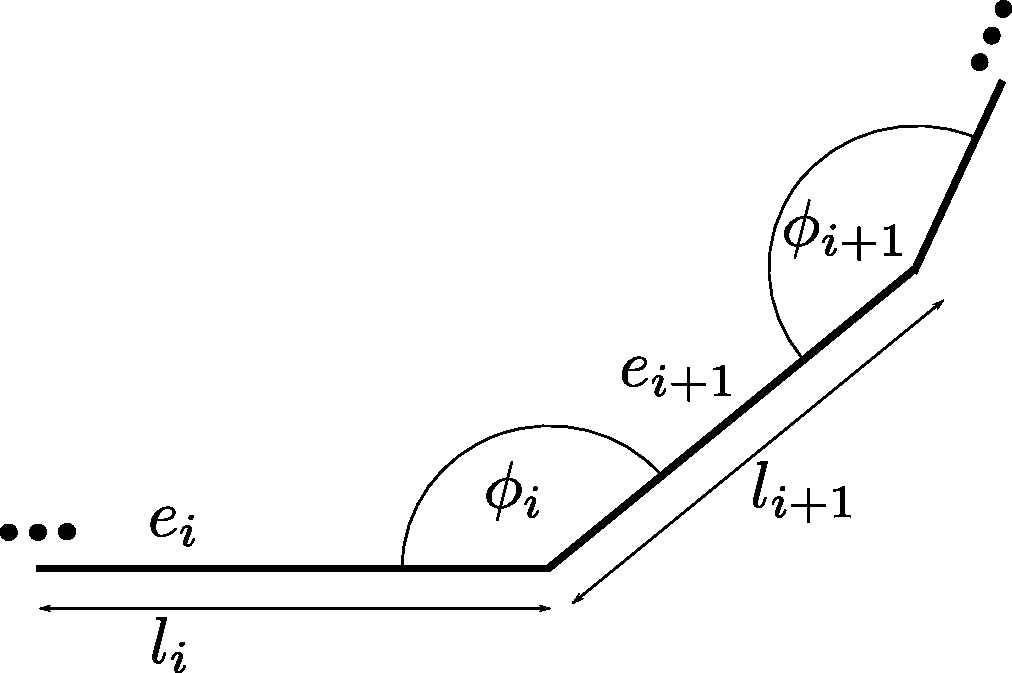
\includegraphics[width=0.4\textwidth]{convPolygon.pdf}
  \caption{Convex polygon with edges $e_i$ length $l_i$ and interior angles $\phi_i$.}
  \label{fig:convPol}
\end{figure}

\begin{lemma} \label{Lemma:convexPolMap}
Assume that the robot bounces at angle $\theta$ between adjacent edges $e_i$ and $e_{(i+1)\bmod n}$. Define the constrained bounce map $b^+_{\theta} : (0, l_i) \to (0, l_i)$, such that it makes the robot bounce $m$ times from $e_i$ back to $e_i$, and maps $x$, the robot's distance from vertex $v_i$, to $b^+_{\theta}(x)$ distance again from $v_i$. This mapping function is given by
\begin{equation} \label{eq:b-m-bounce}
b^+_{\theta}(x) = \sum_{j=0}^{m-1}(-1)^{m-1-j} l_{(i+j)\bmod n} \prod_{k=j}^{m-1} \mathrm{C}_{(i+k)\bmod n} + (-1)^{m}x \prod_{k=0}^{m-1} \mathrm{C}_{(i+k)\bmod n}
\end{equation}
in which $\mathrm{C}_{j}=\cos(\theta) / \cos(\theta - \phi_j)$.
\end{lemma}
\begin{proof}
If the robot bounces at fixed angle $\theta$, the map between edges $e_i$ and $e_{(i+1)\bmod n}$ is given by $\mathrm{\textbf{b}}(l_i,\phi_i) = \frac{ \cos(\theta)}{\cos( \theta - \phi_i)} (l_i - x)$. Let $\mathrm{C}_{i} = \cos( \theta - \phi_i)$. Bouncing $m$ times through consecutive edges corresponds to composing $\mathrm{\textbf{b}}(l_i,\phi_i)$ $m-1$ times, which yields

\begin{equation*}
\mathrm{\textbf{b}}(l_{i+m-1},\phi_{i+m-1}) \circ \mathrm{\textbf{b}}(l_{i+m-2},\phi_{i+m-2}) \circ ... \circ \mathrm{\textbf{b}}(l_i,\phi_i) 
\end{equation*}
\begin{align*}
&= \mathrm{C}_{i+m-1}(l_{i+m-1} - (\mathrm{C}_{i+m-2} (l_{i+m-2} - ... -  \mathrm{C}_i(l_i - x)...))) \\
&= \mathrm{C}_{i+m-1} l_{i+m-1} - \mathrm{C}_{i+m-1} \mathrm{C}_{i+m-2} l_{i+m-2} + ...  \mathrm{C}_{i+m-1} ... \mathrm{C}_{i+1} \mathrm{C}_{i} (l_i - x_i) 
\end{align*}
Grouping the terms in the last expression yields Equation~(\ref{eq:b-m-bounce}).  

\end{proof}


\begin{remark} \label{rm1}
Note that $m \in \{1,2...,n\}$. In the case of regular $n$-sided polygons, setting $m=1$ correctly models a bounce map between consecutive edges, as $l_i=l_j$ and $\phi_i=\phi_j$, $\forall i,j \in \{0,1,..,n-1\} $.   
\end{remark}



\begin{lemma} \label{Lemma:convexPolContrMap}
If $\abs{\;\prod_{k=0}^{m-1} \mathrm{C}_{(i+k)\bmod n}} < 1$, then $b^+_{\theta}(x)$ is a contraction mapping and has a unique fixed point.
\end{lemma}
\begin{proof}
In order for $b^+_{\theta}(x)$ to be a contraction mapping with a unique fixed point, we check that $ d(b^+_{\theta}(x), b^+_{\theta}(y)) \leq k d(x,y) $ for all $x, y \in (0,l)$ and some nonnegative real number $0 \leq k < 1$.
\begin{equation*}
d(b^+_{\theta}(x), b^+_{\theta}(y))
\end{equation*}
\begin{align*}
	& = \bigg| \sum_{j=0}^{m-1}(-1)^{m-1-j} l_{(i+j)\bmod n} \prod_{k=j}^{m-1} \mathrm{C}_{(i+k)\bmod n} + (-1)^{m}x \prod_{k=0}^{m-1} \mathrm{C}_{(i+k)\bmod n} \\ 
	& - \sum_{j=0}^{m-1}(-1)^{m-1-j} l_{(i+j)\bmod n} \prod_{k=j}^{m-1} \mathrm{C}_{(i+k)\bmod n} - (-1)^{m}y \prod_{k=0}^{m-1} \mathrm{C}_{(i+k)\bmod n} \bigg|  \\
    & = \abs{ (-1)^{m} \prod_{k=0}^{m-1} \mathrm{C}_{(i+k)\bmod n} (x-y)} \\
	& = \abs{\prod_{k=0}^{m-1} \mathrm{C}_{(i+k)\bmod n}} d(x,y).
\end{align*}

Thus if $\abs{\;\prod_{k=0}^{m-1} \mathrm{C}_{(i+k)\bmod n}} < 1$, then $b^+_{\theta}$ is a contraction mapping, and by the Banach fixed-point
theorem, it has a unique fixed point.
\end{proof}





\begin{theorem} \label{Theorem:cycleExistence}
In every convex $n$-sided polygon, there exists a range for $\theta$ such that iterating $b^+_{\theta}(x)$ results in a stable limit cycle of period $n$, which strikes $e_i$ at point distance $x_{FP}$ from vertex $v_i$. Distance $x_{FP}$ is given by
\begin{equation} \label{eq:conPolFP}
x_{FP} = \frac{ \sum_{j=0}^{m-1}(-1)^{m-1-j} l_{(i+j)\bmod n} \prod_{k=j}^{m-1} \mathrm{C}_{(i+k)\bmod n} }{1- (-1)^{m} \prod_{k=0}^{m-1} \mathrm{C}_{(i+k)\bmod n}}
\end{equation}
\noindent in which $\mathrm{C}_{j}=cos(\theta) / cos(\theta - \phi_j)$, and $\theta \in (\min\{\phi_i / 2 \}, \pi/2 )$.
\end{theorem}
\begin{proof}
The function $b^+_{\theta}$ given in Lemma~\ref{Lemma:convexPolMap} describes a robot that bounces at angle $\theta$ between adjacent edges $e_i$ and $e_{(i+1)\bmod n}$ in a convex $n$-gon, beginning its trajectory at a point $p \in P$ which is at a distance $x$ from $v_i$. If the robot is constrained to hit adjacent walls, then $\theta$ must be greater than  $\min\{\phi_i / 2 \}$ and less than $\pi/2$. Setting $\theta \in (\min\{\phi_i / 2 \}, \pi/2 )$ also yields $\abs{\;\prod_{k=0}^{m-1} \mathrm{C}_{(i+k)\bmod n}} < 1$, hence, by Lemma~\ref{Lemma:convexPolContrMap}, $b^+_{\theta}(x)$ has a unique fixed point, which is an orbit of $B_\theta$ since the robot keeps contacting $e_i$ at the same distance from $v_i$ every time it returns to it. 

To get the fixed point $x_{FP}$ equate Equation~(\ref{eq:b-m-bounce}) to $x$, and solve for $x$ yielding Equation~(\ref{eq:conPolFP}). The result follows.
\end{proof}

\end{document}